% Options for packages loaded elsewhere
\PassOptionsToPackage{unicode}{hyperref}
\PassOptionsToPackage{hyphens}{url}
%
\documentclass[
  12pt,
  landscape]{article}
\usepackage{lmodern}
\usepackage{amssymb,amsmath}
\usepackage{ifxetex,ifluatex}
\ifnum 0\ifxetex 1\fi\ifluatex 1\fi=0 % if pdftex
  \usepackage[T1]{fontenc}
  \usepackage[utf8]{inputenc}
  \usepackage{textcomp} % provide euro and other symbols
\else % if luatex or xetex
  \usepackage{unicode-math}
  \defaultfontfeatures{Scale=MatchLowercase}
  \defaultfontfeatures[\rmfamily]{Ligatures=TeX,Scale=1}
\fi
% Use upquote if available, for straight quotes in verbatim environments
\IfFileExists{upquote.sty}{\usepackage{upquote}}{}
\IfFileExists{microtype.sty}{% use microtype if available
  \usepackage[]{microtype}
  \UseMicrotypeSet[protrusion]{basicmath} % disable protrusion for tt fonts
}{}
\makeatletter
\@ifundefined{KOMAClassName}{% if non-KOMA class
  \IfFileExists{parskip.sty}{%
    \usepackage{parskip}
  }{% else
    \setlength{\parindent}{0pt}
    \setlength{\parskip}{6pt plus 2pt minus 1pt}}
}{% if KOMA class
  \KOMAoptions{parskip=half}}
\makeatother
\usepackage{xcolor}
\IfFileExists{xurl.sty}{\usepackage{xurl}}{} % add URL line breaks if available
\IfFileExists{bookmark.sty}{\usepackage{bookmark}}{\usepackage{hyperref}}
\hypersetup{
  hidelinks,
  pdfcreator={LaTeX via pandoc}}
\urlstyle{same} % disable monospaced font for URLs
\usepackage[margin=1in]{geometry}
\usepackage{graphicx,grffile}
\makeatletter
\def\maxwidth{\ifdim\Gin@nat@width>\linewidth\linewidth\else\Gin@nat@width\fi}
\def\maxheight{\ifdim\Gin@nat@height>\textheight\textheight\else\Gin@nat@height\fi}
\makeatother
% Scale images if necessary, so that they will not overflow the page
% margins by default, and it is still possible to overwrite the defaults
% using explicit options in \includegraphics[width, height, ...]{}
\setkeys{Gin}{width=\maxwidth,height=\maxheight,keepaspectratio}
% Set default figure placement to htbp
\makeatletter
\def\fps@figure{htbp}
\makeatother
\setlength{\emergencystretch}{3em} % prevent overfull lines
\providecommand{\tightlist}{%
  \setlength{\itemsep}{0pt}\setlength{\parskip}{0pt}}
\setcounter{secnumdepth}{-\maxdimen} % remove section numbering
\usepackage{dcolumn}
\usepackage{float}
\usepackage{graphicx}
\usepackage{amsmath}

\author{}
\date{\vspace{-2.5em}}

\begin{document}

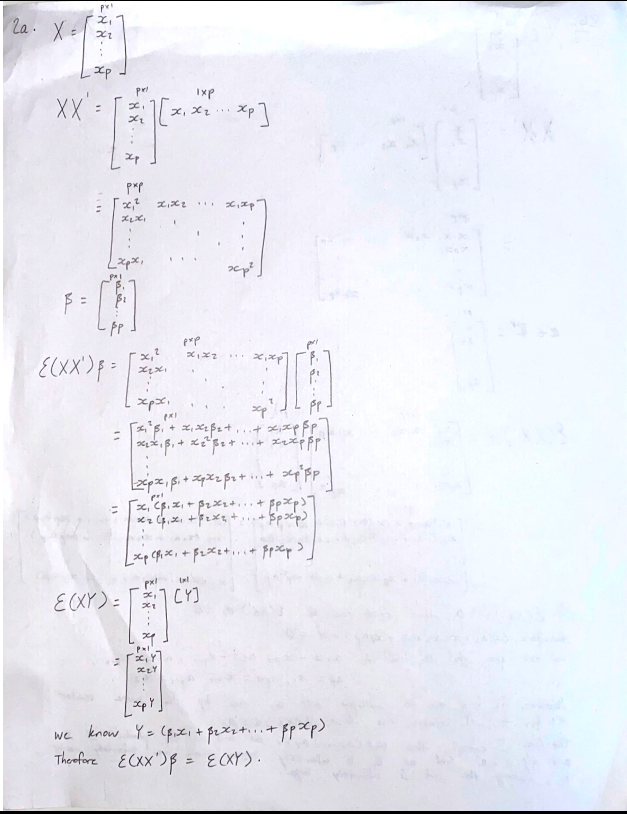
\includegraphics{/users/matthewogle/ds-metrics/pset1/2a.png}
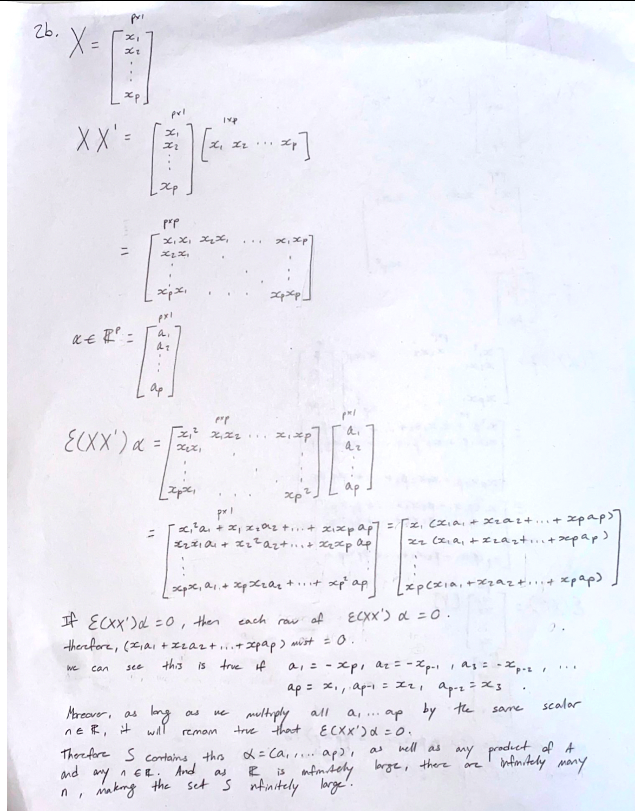
\includegraphics{/users/matthewogle/ds-metrics/pset1/2b.png}

\begin{enumerate}
\def\labelenumi{(\alph{enumi})}
\setcounter{enumi}{2}
\item
\end{enumerate}

No.~Given that we know \(\beta_0\) is the output of a regression using
OLS, it is the result of a minimization problem so there should not be
any other coefficient (not equal to 0) that also satisfies the equation.

\begin{enumerate}
\def\labelenumi{(\alph{enumi})}
\setcounter{enumi}{3}
\item
\end{enumerate}

\begin{enumerate}
\def\labelenumi{\roman{enumi})}
\item
\end{enumerate}

Y is wages

\begin{enumerate}
\def\labelenumi{\roman{enumi})}
\setcounter{enumi}{1}
\item
\end{enumerate}

With in X there are two explanatory variables:

\(X_1\) is age

\(X_2\) is the years of experience in the workforce

\begin{enumerate}
\def\labelenumi{\roman{enumi})}
\setcounter{enumi}{2}
\item
\end{enumerate}

\(X_1\) (Age) has an interesting relationship with wages because as you
get older, you tend to have spent longer at any given job or company,
and you are also seen as more mature and wise. This loyalty and those
respected traits usually result in higher wages.

\(X_2\) (Experience) also has an interesting relationship with wages
because the more experience you have, the more time you spend perfecting
the skills related to the field. If you have spent a longer time within
a certain industry too, you are also likely to be seen as more capable
and worthy of promotions within the industry too. These factors both
make one a more attractive employee, and typically, a more highly paid
employee as well.

\begin{enumerate}
\def\labelenumi{\roman{enumi})}
\setcounter{enumi}{3}
\item
\end{enumerate}

It is unlikely that, even knowing the probability distribution of (X,Y),
we could measure the ``true'' population regression coefficient.
Regressions can never truly measure the exact coefficient, but just do
their best to estimate. However, because there is multicollinearity in
our model, it is even more difficult to measure the ``true'' population
regression coefficient. With multicollinearity, there is less
independent variation for our explanatory variables, ie. we can't see
the effect of age without the effect of experience (and vice versa). The
estimators for age and experience are in a sense ``diluted'' as their
correlation means the effect of age on wage likely captures a portion of
the effect of experience on wage because it is hard to find changes in
age without corresponding changes in experience (and vice versa). For
example we might learn that years of education and years of experience
are both positively correlated with wages. But because the variance of
the estimators are high we don't know exactly how much each contributes
to increasing or decreasing wages.

Problem 3

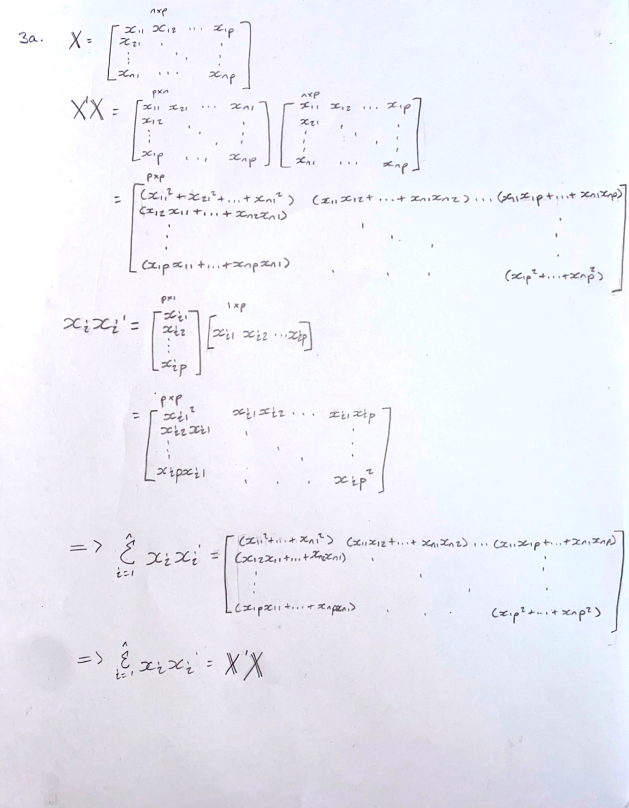
\includegraphics{/users/matthewogle/ds-metrics/pset1/3a.png}
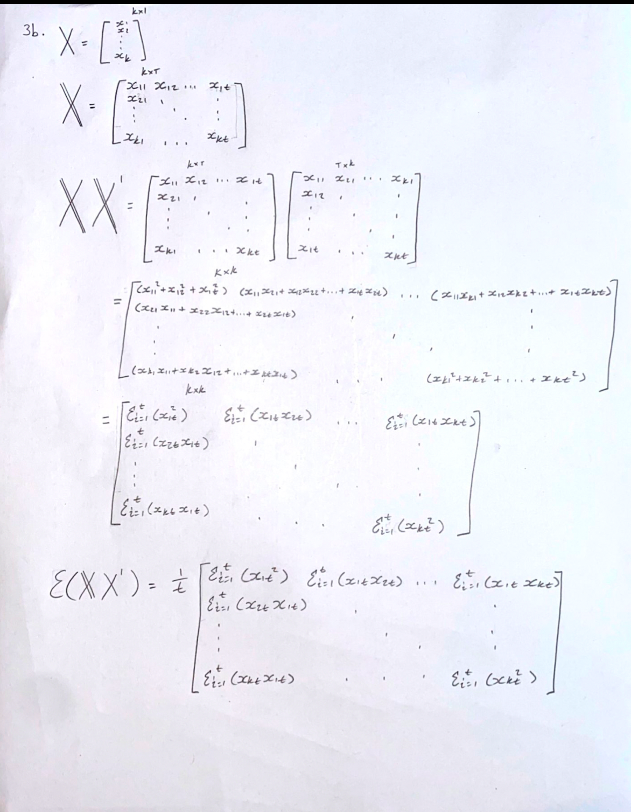
\includegraphics{/users/matthewogle/ds-metrics/pset1/3b.png}

\end{document}
